\subsection{\atmel Modules}
The modules based on the \atmega chip are small boards we designed to take in commands from the main \olimex board via \rsserial and do all of the sensing and switching.

\subsubsection{Sensing}
Current sensing is achived using the \allegro chip manufactured by Allegro Microsystems. The \allegro is a fully integrated, Hall effect based current sensor IC. The chip can sense bidirectional currents of up to \SI{20}{\ampere} with a sensitivity of \SI{100}{\milli\volt\per\ampere} over the whole 0-5V range of its analog output. Coupled with the \atmega 's 10-bit ADC, this gives us a resolution of \SI{48}{\milli\ampere}. One of the more attractive features of the \allegro chip is its \SI{2.1}{\kilo\volt} isolation which dispenses us from adding opto-isolators to the board.\\

\begin{figure}
\centering
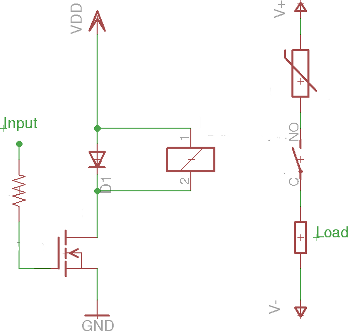
\includegraphics[width=0.5\textwidth,viewport=0 0 995 737]{figures/relaycircuit.png}
\caption{Relay Circuit}
\label{fig:relaycircuit}
\end{figure}

\subsubsection{Switching}
Switching is achieved with two \relay relays manufactured by \relaymf. Since one of the specifications of \netlets is to be able to handle any load that a conventional power strip can, the chosen relay needs to be able to switch high ampere AC loads while keeping cost to a minimum. Solid state relays were not used because ones with a high ampere rating are expensive and the fast switching speed is not necessary for this application. The electromechanical relay is best suited for \netlets because it can handle high voltage/current loads, is relatively inexpensive, and also provides galvanic isolation so AC and DC currents can be placed on the same board. \\

The relays are switched by a \vddval difference across the relay coil terminals. This is acheived by holding one terminal at \vdd and connecting the other end to \transistor power transistor manufactured by \transistormf. A diode is also connected across the terminals to prevent damage to the transistor due to the back-EMF pulse generated when the relay coil is turned off. \fig{fig:relaycircuit} shows this schematic. \\

\subsubsection{Programming, Communication, and Power}
Besides sensing and switching, the board supplies infrastructure for programming and communication, as well as power distribution.
\\An SPI header was added on the prototype for use with an AVR JTAGICE mkII or any other compatible programmer. While useful for debugging, the SPI header would probably be removed from retail versions of the product to lower the hardware costs.
\\RS232 is used for communication. It is chosen over plain UART for its robustness to degradation over relatively long distances. The \shiftr level shifter was chosen to convert UART to RS232 for its low price and high ESD protection. We also included a male DB9 header to allow for the use of null-modem cable. Ideally, this system will be replaced by the zigbee wireless protocol in the future.
\\All of the components require \SI{5}{\volt} to operate properly. Because of prior expectations to have an accompanying power supply board which would do the AC/DC conversion and step down the voltage, only a power header was added to the \atmel module. Regulated power has to be supplied from either another board or a regulated power supply.
% proof of concept modular

\subsubsection{Software}

%%% Local Variables: 
%%% mode: latex
%%% TeX-master: "../netlets"
%%% End: 
